\section{Funciones armónicas}
\subsection{Funciones armónicas}

Vamos a aplicar lo que sabemos de variable compleja al estudio de ecuaciones diferenciables en $\mathbb{R}^2$. En particular, queremos hallar y estudiar las soluciones de las ecuaciones  
\[
    \frac{\partial^2 u}{\partial x^2} + \frac{\partial^2 u}{\partial y^2} = 0
\]
en cierto $\Omega \subset \mathbb{R}^2$ y también hallar soluciones de 
\[
    \begin{cases}
        \frac{\partial^2 u}{\partial x^2} + \frac{\partial^2 u}{\partial y^2} = 0 & \text{en } D(0,1) \\
        h(x,y) = \varphi(x,y) & \forall (x,y) \in \partial D(0,1)
    \end{cases}
\]
Dado $\Omega \subset \mathbb{R}^2$ abierto conexo buscamos funciones $u:\Omega \to \mathbb{R}^2$ de clase $\mathcal{C}^2$ que satisfagan
\[
    \frac{\partial^2 u}{\partial x^2} (x,y) + \frac{\partial^2 u}{\partial y^2} (x,y) = 0 \quad \forall (x,y) \in \Omega.
\]
o escrito abreviadamente que cumplan
\[
    u_{xx} + u_{yy} = 0 \text{ en } \Omega.
\]
A la ecuación anterior se le llama \textbf{ecuación de Laplace} y a sus soluciones en $\Omega$ se les llama \textbf{funciones armónicas} en $\Omega$.

\begin{proposición}
    Si $\Omega \subset \mathbb{C}$ es dominio y $f:\Omega \to \mathbb{C}$ es holomorfa, entonces las funciones $u = \Re(f)$ y $v = \Im(f)$ son armónicas en $\Omega$.
\end{proposición}

\begin{proof}
    Sea $f = u + iv$ con $u,v:\Omega \to \mathbb{R}$. Como $f$ es holomorfa, $u$ y $v$ son diferenciables y verifican las ecuaciones de Cauchy-Riemann en $\Omega$:
    \[
        u_x = v_y \quad u_y = -v_x.
    \]
    Además, tenemos
    \[
        f'(z) = u_x(z) - iu_y(z) = v_y(z) + iv_x(z).
    \]
    Como $f'(z) \in \mathcal{H}(\Omega)$, tenemos que $u_x$, $u_y$, $v_x$ y $v_y$ son diferenciables en $\Omega$ y teniendo en cuenta que $f$ es infinitamente diferenciable en $\Omega$, deducimos que $u$ y $v$ son de clase $\mathcal{C}^\infty$ en $\Omega$.
    Ahora derivando las ecuaciones de Cauchy-Riemann, obtenemos
    \[
        \begin{cases}
            u_{xx} = (v_y)_x = v_{yx} \\
            u_{yy} = (-v_x)_y = -v_{xy} \underbrace{=}_{\text{Schwarz}} -v_{yx} 
        \end{cases}
    \]
    luego $u_{xx} + u_{yy} = 0$ en $\Omega$. Por lo tanto $u$ es armónica en $\Omega$. Para demostrar que $v$ es armónica, se hace de forma análoga o bien se aplica lo que acabamos de probar a la función $-if$.
\end{proof}

\ejemplo{
    \begin{enumerate}
        \item Si $\alpha \in \mathbb{R}$, sabemos que la función $f(z) = e^{\alpha z} \in \mathcal{H}(\mathbb{C})$. Por lo tanto, las funciones
        \[
            u(x,y) = e^{\alpha x} \cos(\alpha y) \quad \text{y} \quad v(x,y) = e^{\alpha x} \sin(\alpha y)
        \]
        son armónicas en $\mathbb{R}^2$.
        \item La función $f(z) = \log(z)$ es holomorfa en $\mathbb{C} \setminus (-\infty,0]$. Por lo tanto, las funciones
        \[
            u(x,y) = \log(\sqrt{x^2 + y^2}) = \frac{1}{2} \log(x^2 + y^2)
        \]
        es armónica en $\mathbb{R}^2 \setminus (-\infty,0]$. De hecho, lo es en $\mathbb{R}^2 \setminus \{(0,0)\}$.
    \end{enumerate}
}

\begin{proposición}
    Si $\Omega \subset \mathbb{C}$ es dominio y $f \in \mathcal{H}(\Omega)$, entonces $\Re(f)$ y $\Im(f)$ son armónicas en $\Omega$.
\end{proposición}

\begin{proof}
    Es fácil comprobar que 
    \begin{itemize}
        \item Si $u_1,u_2$ son armónicas en $\Omega \subset \mathbb{R}^2$ abierto conexo entonces $\alpha u_1 + \beta u_2$ es armónica en $\Omega$ para todo $\alpha,\beta \in \mathbb{R}$.
    \end{itemize}
\end{proof}

\begin{definición} [Función conjugada armónica]
    Si $u:\Omega \to \mathbb{R}$ es armónica en $\Omega \subset \mathbb{R}^2$ abierto conexo, diremos que $v:\Omega \to \mathbb{R}$ es una \textbf{función conjugada armónica} de $u$ en $\Omega$ si la función $f:\Omega \to \mathbb{C}$ dada por $f(z) = u(x,y) + iv(x,y)$ es holomorfa en $\Omega$.
\end{definición}

\begin{teorema}
    Sea $\Omega \subset \mathbb{R}^2$ abierto conexo y sea la función $u:\Omega \to \mathbb{R}$ armónica en $\Omega$. Entonces, para cada $(x_0,y_0) \in \Omega$ existe un entorno abierto conexo $U \subset \Omega$ de $(x_0,y_0)$ y una función $f \in \mathcal{H}(U)$ tal que
    \[
        u(x,y) = \Re(f(x+iy)) \quad \forall (x,y) \in U.
    \]
    Además, si $\Omega$ es simplemente conexo, entonces existe $f \in \mathcal{H}(\Omega)$ tal que
    \[
        u(x,y) = \Re(f(x+iy)) \quad \forall (x,y) \in \Omega.
    \]
    \label{teo:teo_funcion_conjugada_armonica}
\end{teorema}

\begin{proof}
    Suponemos en primer lugar que $\Omega$ es simplemente conexo. Consideramos la siguiente función
    \[
        g(z) = u_x(z) - iu_y(z) \quad \forall z \in \Omega.
    \]
    Como $u$ es armónica en $\Omega$, tenemos que $u_x$ y $-u_y$ son diferenciables en $\Omega$ y además
    \[  
        \begin{matrix}
            (\Re(g))_x = (u_x)_x = u_{xx} \\
            (\Re(g))_y = (u_x)_y = u_{xy} \\
            (\Im(g))_x = (-u_y)_x = -u_{yx} \\
            (\Im(g))_y = (-u_y)_y = -u_{yy}
        \end{matrix}
    \]
    $u$ es armónica luego $u_{xx} + u_{yy} = 0$ en $\Omega$. Por lo tanto, usando el lema de Schwarz, tenemos
    \[
        (\Re(g))_x = u_{xx} = -u_{yy} = (\Im(g))_y
    \]
    \[
        (\Re(g))_y = u_{xy} = u_{yx} = -(-u_{yx}) = -(\Im(g))_x
    \]
    Como $\Re(g)$ y $\Im(g)$ son diferenciables en $\Omega$ y verifican las ecuaciones de Cauchy-Riemann, deducimos que $g \in \mathcal{H}(\Omega)$.
    Luego 
    \[
        \begin{cases}
            g \in \mathcal{H}(\Omega) \\
            \Omega \text{ es simplemente conexo}
        \end{cases} \implies g \text{ tiene primitiva en } \Omega. 
    \]
    Fijamos un $z_0 \in \Omega$ y sea $f$ la primitiva de $g$ en $\Omega$ tal que $f(z_0) = u(z_0)$. Entonces esta $f$ es la que buscamos ya que 
    \[
        f(z) = f_1(z) + if_2(z) \implies g(z) = f'(z) = (\Re(f))_x - i(\Re(f))_y.
    \]
    con lo cual
    \[
        \begin{cases}
            u_x = (\Re(f))_x \\
            v_y = (\Re(f))_y
        \end{cases} \text{ en } \Omega \implies u = \Re(f) + cte \text{ en } \Omega.
    \]
    Como $u(z_0) = \Re(f)(z_0) + cte = u(z_0) + cte$, deducimos que $cte = 0$ y por lo tanto $u = \Re(f)$ en $\Omega$.\\
    En general, si $z_0 \in \Omega$ entonces existe $r > 0$ tal que $D(z_0,r) \subset \Omega$, luego aplicando lo anterior a $D(z_0,r)$ (que es simplemente conexo) obtenemos que existe $f \in \mathcal{H}(D(z_0,r))$ tal que $u = \Re(f)$ en $D(z_0,r)$.
\end{proof}

Vimos en el \cref{teo:teo_funcion_conjugada_armonica}, que si $u$ es una función armónica en un abierto simplemente conexo, entonces $u$ es la parte real de una función holomorfa en dicho abierto. Veamos ahora algunas consecuencias de este hecho.\\
\begin{itemize}
    \item Si $u$ es armónica en un abierto simplemente conexo $\Omega \subset \mathbb{R}^2$, entonces $u$ es de clase $\mathcal{C}^\infty$ en $\Omega$.
    \item Si $u$ es armónica en un abierto simplemente conexo $\Omega \subset \mathbb{R}^2$, y $h: G \to U$ es una función holomorfa con derivada no nula en $G \subset \mathbb{C}$ dominio, entonces la función $v = u \circ h$ es armónica en $G$.\\
    Sea $z_0 \in G$, como $h'(z_0) \neq 0$, por el teorema de la función inversa, existe un entorno abierto $U$ de $z_0$ tal que $h|_U: U \to h(U)$ es biholomorfa. Llamemos $w_0 = h(z_0) \in h(U) \subset \Omega$. Como $h(U)$ es abierto, existe $r > 0$ tal que $D(w_0,r) \subset h(U)$. Por el \cref{teo:teo_funcion_conjugada_armonica}, existe $f \in \mathcal{H}(D(w_0,r))$ tal que $u = \Re(f)$ en $D(w_0,r)$. Tomando $U_1 = h^{-1}(D(w_0,r)) \subset U$, tenemos que $U_1$ es un entorno abierto de $z_0$ y
    \[
        v(z) = (u \circ h)(z) = \Re((f \circ h)(z)) \quad \forall z \in U_1.
    \]
    Como $z_0$ es arbitrario, deducimos que $v$ es armónica en $G$.
\end{itemize}

Para las funciones armónicas no tenemos un principio de identidad como en el caso de las funciones holomorfas. Por ejemplo, la función $u(x,y) = \log(x^2 + y^2)$ es armónica en $\mathbb{R}^2 \setminus \{(0,0)\}$ y se anula para todo $(x,y) \in C(0,1)$. La circunferencia $C(0,1)$ tiene muchos puntos de acumulación en $\mathbb{R}^2 \setminus \{(0,0)\}$ pero $u$ no es idénticamente cero en dicho conjunto. Sin embargo, sí que tenemos el siguiente resultado.

\begin{teorema}
    Sea $\Omega \subset \mathbb{R}^2$ un dominio y sean $u_1,u_2:\Omega \to \mathbb{R}$ funciones armónicas en $\Omega$. Si $u_1 \equiv u_2$ en un disco $D \subset \Omega$, entonces $u_1 \equiv u_2$ en todo $\Omega$.
\end{teorema}

\begin{proof}
    Supongamos en primer lugar que $\Omega$ es simplemente conexo. Como $u_1$ y $u_2$ son armónicas en $\Omega$, entonces tenemos que $u_1 - u_2$ es armónica en $\Omega$. Por el \cref{teo:teo_funcion_conjugada_armonica}, existe $f \in \mathcal{H}(\Omega)$ tal que
    \[
        u_1(x,y) - u_2(x,y) = \Re(f(x+iy)) \quad \forall (x,y) \in \Omega.
    \]
    Si $u_1 \equiv u_2$ en un disco $D \subset \Omega$, entonces $u_1-u_2 \equiv 0$ en $D$, luego $\Re(f(z)) = 0$ para todo $z \in D$. Así, tenemos que $f$ es constante en $D \implies \Re(f) \equiv 0$ en $\Omega$ (por ser $\Re(f) \equiv 0$ en $D$), y por el principio de identidad para funciones holomorfas, deducimos que $f \equiv 0$ en $\Omega$. Por lo tanto, $u_1 \equiv u_2$ en $\Omega$.\\
    Ahora veamos el caso general: $\Omega$ es abierto conexo.\\
    Sea 
    \[
        B = \{z \in \Omega : \exists r > 0 \text{ tal que } D(z,r) \subset \Omega \text{ y } u_1 \equiv u_2 \text{ en } D(z,r)\}.
    \]
    entonces tenemos que $B \neq \emptyset$ ya que el centro del disco $D$ pertenece a $B$. Veamos que $B$ es abierto. Si $z_0 \in B$, existe $r_0 > 0$ tal que $D(z_0,r_0) \subset \Omega$ y $u_1 \equiv u_2$ en $D(z_0,r_0)$. Para cada $z \in D(z_0,r_0)$, existe $r_z > 0$ tal que $D(z,r_z) \subset D(z_0,r_0) \subset \Omega$. Y como $u_1 \equiv u_2$ en $D(z_0,r_0)$, tenemos que $u_1 \equiv u_2$ en $D(z,r_z)$. Por lo tanto, $z \in B$. Hemos probado que $D(z_0,r_0) \subset B$, luego $B$ es abierto.\\
    Veamos que $B$ es cerrado en $\Omega$. Sea $(z_n)_{n \in \mathbb{N}} \subset B$ una sucesión que converge a $z_0 \in \Omega$. Queremos probar que $z_0 \in B$. Como $z_0 \in \Omega$ abierto, existe $R > 0$ tal que $D(z_0,R) \subset \Omega$. Como $z_n \to z_0$, existe $N \in \mathbb{N}$ tal que $z_n \in D(z_0,R/2)$ para todo $n \geq N$. En particular, $z_N \in B$, luego existe $r_N > 0$ tal que $D(z_N,r_N) \subset \Omega$ y $u_1 \equiv u_2$ en $D(z_N,r_N)$.\\
    Tomamos $\delta > 0$ tal que
    \[
        D(z_N,\delta) \subset D(z_N,r_N) \cap D(z_0,R).
    \]
    Entonces, tenemos que $u_1 \equiv u_2$ en $D(z_N,\delta)$. Además, como $D(z_N,\delta) \subset D(z_0,R)$ (este último simplemente conexo), por el primer caso, deducimos que $u_1 \equiv u_2$ en $D(z_0,R)$. Por lo tanto, $z_0 \in B$ y hemos probado que $B$ es cerrado en $\Omega$.\\
    Como $B \neq \emptyset$, $B$ es abierto y cerrado en $\Omega$ y $\Omega$ es conexo, deducimos que $B = \Omega$.\\
    Fijamos entonces $z_1 \in D$, para cada $z \in \Omega$, como $\Omega$ es conexo por caminos (por ser abierto y conexo), existe un camino $\gamma$ en $\Omega$ que une $z_1$ con $z$. Para cada punto de $\gamma^*$, sabemos que existe un disco centrado en él tal que las funciones $u_1$ y $u_2$ coinciden en dicho disco. Usando la compacidad de $\gamma^*$, podemos cubrir $\gamma^*$ con un número finito de estos discos $D_1, \ldots, D_m$ tales que $z_1 \in D_1$ y $z \in D_m$ y además $D_j \cap D_{j+1} \neq \emptyset$ para $j = 1, \ldots, m-1$ y tale que $u_1 \equiv u_2$ en cada $D_j$ para $j = 1, \ldots, m$. De aquí deducimos que $u_1(z) = u_2(z)$ y como $z$ es arbitrario, tenemos que $u_1 \equiv u_2$ en $\Omega$.\\
    Probado que $B = \{z \in \Omega : u_1(z) = u_2(z)\} = \Omega$, ya hemos terminado, pues si $z \in \Omega$, entonces $z \in B$ y por lo tanto $u_1(z) = u_2(z)$.
\end{proof}

\begin{teorema} [Teorema del valor medio para funciones armónicas]
    Sea $\Omega \subset \mathbb{R}^2$ un dominio y sea $u:\Omega \to \mathbb{R}$ una función armónica en $\Omega$. Entonces, para cada $z_0 \in \Omega$ y cada $r > 0$ tal que $\overline{D}(z_0,r) \subset \Omega$, se cumple que
    \[
        u(z_0) = \frac{1}{2\pi} \int_0^{2\pi} u(z_0 + re^{it}) dt.
    \]
\end{teorema}

\begin{proof}
    Sea $r > 0$ tal que $\overline{D}(z_0,r) \subset \Omega$. Entonces $\exists \delta > 0$ tal que $D(z_0,r + \delta) \subset \Omega$. La función $u$ es armónica en $D(z_0,r + \delta)$, y $D(z_0,r + \delta)$ es simplemente conexo, luego por el \cref{teo:teo_funcion_conjugada_armonica}, existe $f \in \mathcal{H}(D(z_0,r + \delta))$ tal que
    \[
        u(z) = \Re(f(z)) \quad \forall z \in D(z_0,r + \delta).
    \]
    Por la fórmula integral de Cauchy, tenemos que
    \[
        f(z_0) = \frac{1}{2\pi i} \int_{C(z_0,r)} \frac{f(w)}{w - z_0} dw = \frac{1}{2\pi} \int_0^{2\pi} \frac{f(z_0 + re^{it})}{re^{it}} ire^{it} dt = \frac{1}{2\pi} \int_0^{2\pi} f(z_0 + re^{it}) dt.
    \]
    con lo cual
    \[
        u(z_0) = \Re(f(z_0)) = \Re\left(\frac{1}{2\pi} \int_0^{2\pi} f(z_0 + re^{it}) dt\right) = \frac{1}{2\pi} \int_0^{2\pi} \Re(f(z_0 + re^{it})) dt = \frac{1}{2\pi} \int_0^{2\pi} u(z_0 + re^{it}) dt.
    \]
\end{proof}

\begin{teorema} [Principio del máximo para funciones armónicas]
    Sea $\Omega \subset \mathbb{R}^2$ un dominio y sea $u:\Omega \to \mathbb{R}$ una función armónica en $\Omega$. Si $u$ no es constante en $\Omega$, entonces $u$ no tiene ni máximo ni mínimo locales en $\Omega$.
\end{teorema}

\begin{proof}
    Supongamos que $u$ tiene un máximo local en $z_0 \in \Omega$. Entonces, existe $r > 0$ tal que $\overline{D}(z_0,r) \subset \Omega$ y
    \[
        u(z) \leq u(z_0) \quad \forall z \in D(z_0,r).
    \]
    Por el teorema del valor medio para funciones armónicas, si $\rho \in (0,r)$, se cumple que
    \[
        u(z_0) = \frac{1}{2\pi} \int_0^{2\pi} u(z_0 + \rho e^{it}) dt \leq \frac{1}{2\pi} \int_0^{2\pi} u(z_0) dt = u(z_0).
    \]
    con lo cual 
    \[
        \int_{0}^{2\pi} u(z_0 + \rho e^{it}) dt = \int_0^{2\pi} u(z_0) dt \implies \int_{0}^{2\pi} (u(z_0) - u(z_0 + \rho e^{it})) dt = 0.
    \]
    \[
        \implies u(z_0) - u(z_0 + \rho e^{it}) = 0 \quad \forall t \in [0,2\pi] \implies u(z_0) = u(z_0 + \rho e^{it}) \quad \forall t \in [0,2\pi].
    \]
    teniendo en cuenta que el integrando es constante y positivo.
    Por lo tanto, $u$ es constante en la circunferencia $C(z_0,\rho)$ y esa constante es $u(z_0)$. Como ocurren $\forall \rho \in (0,r)$, deducimos que $u$ es constante en $D(z_0,r)$. Por el teorema 2, tenemos que $u$ es constante en todo $\Omega$. Si $z_1$ es mínimo local de $u$ en $\Omega$, entonces $z_j$ es máximo local de $-u$ en $\Omega$ (pues $-u$ es armónica en $\Omega$), luego $-u$ es constante en $\Omega$ y por lo tanto $u$ es constante en $\Omega$.
\end{proof}

Veamos algunas consecuencias

\begin{corolario}
    Si $u$ es armónica en un dominio acotado $\Omega \subset \mathbb{R}^2$ y es continua en $\overline{\Omega}$, entonces $u$ alcanza sus valores máximo y mínimo en $\partial \Omega$.
\end{corolario}

\begin{proof}
    Si $u$ es constante, entonces alcanza sus valores máximo y mínimo en cualquier punto de $\overline{\Omega}$, en particular en $\partial \Omega$. Si $u$ no es constante, debe alcanzar su valor máximo y mínimo en algún punto de $\overline{\Omega}$ al ser continua en el compacto $\overline{\Omega}$. Por el principio del máximo y del mínimo, $u$ no puede alcanzar ni su máximo ni su mínimo en $\Omega$, luego debe alcanzarlos en $\partial \Omega = \overline{\Omega} \setminus \Omega$.
\end{proof}

\begin{corolario}
    Si $u_1,u_2$ son armónicas en un disco $D \subset \mathbb{R}^2$ y son continuas en $\overline{D}$. Si $u_1 \equiv u_2$ en $\partial D$, entonces $u_1 \equiv u_2$ en $\overline{D}$.
\end{corolario}

\begin{proof}
    Las funciones $u_1$ y $u_2$ son armónicas en $D$, luego $u_1 - u_2$ es armónica en $D$. Además, $u_1 - u_2$ es continua en $\overline{D}$, pues $u_1$ y $u_2$ lo son. Por el corolario anterior, $u_1 - u_2$ alcanza sus valores máximo y mínimo en $\partial D$. Como $u_1 \equiv u_2$ en $\partial D$, tenemos que
    \[
        0 \leq u_1(x,y) - u_2(x,y) \leq 0 \quad \forall (x,y) \in \partial D,
    \]
    luego $u_1(x,y) = u_2(x,y)$ para todo $(x,y) \in \partial D$. 
\end{proof}

\begin{corolario}
    Sean $u_1,u_2$ armónicas en un dominio $\Omega \subset \mathbb{R}^2$ tal que coinciden en la frontera de un disco $D$ con $\overline{D} \subset \Omega$. Entonces, $u_1 \equiv u_2$ en $\overline{D}$.
\end{corolario}

\begin{proof}
    Por el corolario anterior, $u_1 \equiv u_2$ en $\overline{D}$. Por otro lado, el teorema 2 nos dice que si dos funciones armónicas coinciden en un disco, entonces coinciden en todo el dominio. Por lo tanto, $u_1 \equiv u_2$ en $\Omega$.
\end{proof}

\subsection{El problema de Dirichlet en el disco}

El problema de Dirichlet consiste en dado un dominio $\Omega \subset \mathbb{R}^2$ y una función continua $\varphi:\partial \Omega \to \mathbb{R}$, hallar las funciones $u:\overline{\Omega} \to \mathbb{R}$ tal que
\[
    \begin{cases}
        u \text{ es } \mathcal{C}^2 \text{ y } u_{xx} + u_{yy} = 0 \text{ en } \Omega \\
        u \text{ es continua en } \overline{\Omega} \\
        u = \varphi \text{ en } \partial \Omega
    \end{cases}
\]
o escrito de otra forma
\[
    \begin{cases}
        u \text{ es armónica en } \Omega \\
        u \text{ es continua en } \overline{\Omega} \\
        u = \varphi \text{ en } \partial \Omega
    \end{cases}
\]
Nos interesa saber si existe solución al problema de Dirichlet, cuántas hay y cómo se pueden hallar. 

Recordamos la fórmula integral de Poisson que nos dice que si $f$ es holomorfa en un dominio $\Omega$ que contiene el disco cerrado $\overline{D}(0,1)$, entonces para cada $z = re^{i\theta} \in D(0,1)$, se cumple que
\[
    f(z) = \frac{1}{2\pi} \int_0^{2\pi} \left( \frac{1 - r^2}{1 + r^2 - 2r \cos(\theta - t)} \right) f(e^{it}) dt.
\]

\begin{teorema} [Fórmula integral de Poisson para funciones armónicas]
    Sea $u$ una función armónica en un dominio $\Omega \subset \mathbb{R}^2$ que contiene el disco cerrado $\overline{D}(0,1)$. Entonces, para cada $z = re^{i\theta} \in D(0,1)$, se cumple que
    \[
        u(z) = \frac{1}{2\pi} \int_0^{2\pi} \left( \frac{1 - r^2}{1 + r^2 - 2r \cos(\theta - t)} \right) u(e^{it}) dt.
    \]
\end{teorema}

\begin{proof}
    Tenemos que $\overline{D}(0,1) \subset \Omega$, luego existe $\delta > 0$ tal que $D(0,1 + \delta) \subset \Omega$. La función $u$ es armónica en $D(0,1 + \delta)$, y $D(0,1 + \delta)$ es simplemente conexo, luego por el \cref{teo:teo_funcion_conjugada_armonica}, existe $f \in \mathcal{H}(D(0,1 + \delta))$ tal que
    \[
        u(z) = \Re(f(z)) \quad \forall z \in D(0,1 + \delta).
    \]
    Por tanto, teniendo en cuenta la fórmula integral de Poisson para funciones, tenemos que si $z = re^{i\theta} \in D(0,1)$, se cumple que
    \[
        u(z) = \Re(f(z)) = \Re\left( \frac{1}{2\pi} \int_0^{2\pi} \left( \frac{1 - r^2}{1 + r^2 - 2r \cos(\theta - t)} \right) f(e^{it}) dt \right)
    \]
    \[
        = \frac{1}{2\pi} \int_0^{2\pi} \left( \frac{1 - r^2}{1 + r^2 - 2r \cos(\theta - t)} \right) \Re(f(e^{it})) dt 
        = \frac{1}{2\pi} \int_0^{2\pi} \left( \frac{1 - r^2}{1 + r^2 - 2r \cos(\theta - t)} \right) u(e^{it}) dt.
    \]
\end{proof}

\begin{definición} [Núcleo de Poisson]
    La función $P:[0,1) \times \mathbb{R} \to \mathbb{R}$ dada por
    \[
        P_r(t) = \frac{1 - r^2}{1 + r^2 - 2r \cos(t)} \quad \forall r \in [0,1), \forall t \in \mathbb{R}
    \]
    se llama \textbf{núcleo de Poisson}. Se puede ver como una función en dos variables, $r$ y $t$, o bien como una familia de funciones de una variable $P_r:\mathbb{R} \to \mathbb{R}$ parametrizadas por $r \in [0,1)$.
\end{definición}

La tesis del teorema anterior se puede reescribir como

\[
    u(re^{i\theta}) = \frac{1}{2\pi} \int_0^{2\pi} P_r(\theta - t) u(e^{it}) dt \quad \forall r \in [0,1), \forall \theta \in \mathbb{R}.
\]

\textbf{Propiedades:}
\begin{enumerate}
    \item $P_r(t) > 0$ para todo $r \in [0,1)$ y todo $t \in \mathbb{R}$.
    \item $\displaystyle \frac{1}{2\pi} \int_0^{2\pi} P_r(t) dt = 1$ para todo $r \in [0,1)$.\\
    Basta aplicar la fórmula integral de Poisson a la función constante $f \equiv 1$.
    \[
        P_r(\theta - t) = \Re\left( \frac{e^{it} + z}{e^{it} - z} \right) 
    \]
    en efecto, sea $z \in D(0,1)$, $z = re^{i\theta}$, y llamemos $w = e^{it} \in C(0,1)$, entonces
    \[
        \frac{e^{it} + z}{e^{it} - z} = \frac{(w+z)(\overline{w} - \overline{z})}{|w - z|^2} = \frac{w \overline{w} - z \overline{z} + z \overline{w} - \overline{z} w}{|w - z|^2} = \frac{1 - r^2 + (z \overline{w} - \overline{z \overline{w}})}{|w - z|^2}.
    \]
    \[
        \implies \Re\left( \frac{e^{it} + z}{e^{it} - z} \right) = \frac{1 - r^2}{|w - z|^2} 
    \]
    \[
        |w - z|^2 = |e^{it} - re^{i\theta}|^2 = | (\cos(t) + i \sin(t)) - (r \cos(\theta) + ir \sin(\theta)) |^2 = ((\cos(t) - r \cos(\theta))^2 + (\sin(t) - r \sin(\theta))^2) 
    \] 
    \[
    = 1 + r^2 - 2r (\cos(t) \cos(\theta) + \sin(t) \sin(\theta)) = 1 + r^2 - 2r \cos(\theta - t).
    \]
\end{enumerate}

Recordemos el ejercicio $8$ de la hoja $7$. Si $\varphi$ es continua en $\gamma^*$ con $\gamma$ camino cerrado en $\mathbb{C}$ y definimos
\[
    f(z) := \frac{1}{2\pi i} \int_{\gamma} \frac{\varphi(w)}{w - z} dw \quad \forall z \in \mathbb{C} \setminus \gamma^*,
\]  
entonces $f \in \mathcal{H}(\mathbb{C} \setminus \gamma^*)$ y 
\[
    f'(z) = \frac{1}{2\pi i} \int_{\gamma} \frac{\varphi(w)}{(w - z)^2} dw \quad \forall z \in \mathbb{C} \setminus \gamma^*.
\]

\begin{teorema}
    Sea $\varphi: C(0,1) \to \mathbb{R}$ una función continua y sea la función $u:D(0,1) \to \mathbb{R}$ dada por
    \[
        u(z) := \frac{1}{2\pi} \int_0^{2\pi} \left( \frac{1 - r^2}{1 + r^2 - 2r \cos(\theta - t)} \right) \varphi(e^{it}) dt \quad \forall z = re^{i\theta} \in D(0,1).
    \]
    entonces $u$ define una función armónica en $D(0,1)$ tal que 
    \[
        \lim_{z \to z_0} u(z) = \varphi(z_0) \quad \forall z_0 \in C(0,1).
    \]
\end{teorema}

\begin{proof}
    Sea $\varphi: C(0,1) \to \mathbb{R}$ continua.\\
    Lo primero será ver que $u$ es armónica en $D(0,1)$. Para ello, veamos que es la parte real de una función holomorfa en $D(0,1)$.\\
    Sea $z = re^{i\theta} \in D(0,1)$, ahora tenemos que:
    \[
        u(z) = \frac{1}{2\pi} \int_0^{2\pi} P_r(\theta - t) \varphi(e^{it}) dt = 
        \frac{1}{2\pi} \int_0^{2\pi} \Re\left( \frac{e^{it} + z}{e^{it} - z} \right) \varphi(e^{it}) dt = 
        \Re\left( \frac{1}{2\pi} \int_0^{2\pi} \frac{e^{it} + z}{e^{it} - z} \varphi(e^{it}) dt \right) =
    \]
    \[
        = \Re\left( \frac{1}{2\pi i} \int_{0}^{2\pi} \frac{e^{it} + z}{e^{it} - z} \varphi(e^{it}) \frac{ie^{it}}{e^{it}} dt \right) =
        \Re\left( \frac{1}{2\pi i} \int_{C(0,1)} \frac{w + z}{w - z} \frac{1}{w} \varphi(w) dw \right) \underbrace{=}_{\frac{w+z}{(w-z)w} = \frac{2}{w-z} - \frac{1}{w}}
    \]
    \[
        = \Re\left( \frac{1}{2\pi i} \int_{C(0,1)} \left( \frac{2}{w - z} dw
        - \frac{1}{z} \int_{C(0,1)} \frac{\varphi(w)}{w} dw \right) \right)
        =^*
    \]
    Usemos ahora en $=^*$ el resultado del ejercicio $8$ de la hoja $7$, como $2\varphi$ es continua en $C(0,1)$, la función $f(z) = \frac{1}{2\pi i} \int_{C(0,1)} \frac{2\varphi(w)}{w - z} dw$ es holomorfa en $\mathbb{C} \setminus C(0,1)$, continuemos ahora con la demostración:
    \[
        =^* \Re\left( f(z) - \frac{1}{2\pi i} \int_{C(0,1)} \frac{\varphi(w)}{w} dw \right) = \Re(f(z) - \alpha)
    \]
    Con:
    \[
        \alpha = \frac{1}{2\pi i} \int_{C(0,1)} \frac{\varphi(w)}{w} dw \in \mathbb{C} \text{ constante.}
    \]
    Así, $u(z) = \Re(f(z) - \alpha)$ para todo $z \in D(0,1)$, luego $u$ es la parte real de una función holomorfa en $D(0,1)$ y por lo tanto es armónica en $D(0,1)$.\\
    
    Veamos ahora la 2ª parte de la tesis. Sea $z_0 \in C(0,1)$, queremos ver que:
    \[
        \lim_{z \to z_0} u(z) = \varphi(z_0)
    \]
    Para ello, sea $\varepsilon > 0$, buscamos un $\delta > 0$ tal que si $|z - z_0| < \delta$, entonces $|u(z) - \varphi(z_0)| < \varepsilon$, veamos:
    \[
        |u(z) - \varphi(z_0)| = \left| \frac{1}{2\pi} \int_0^{2\pi} P_r(\theta - t) \varphi(e^{it}) dt - \varphi(z_0) \right| \underbrace{=}_{\frac{1}{2\pi} \int_0^{2\pi} P_r(\theta - t) dt = 1}
    \]
    \[
        = \left| \frac{1}{2\pi} \int_0^{2\pi} P_r(\theta - t) (\varphi(e^{it}) dt - 
        \left( \frac{1}{2\pi} \int_0^{2\pi} P_r(\theta - t) dt \right) \varphi(z_0) \right| =
    \]
    \[
        = \left| \frac{1}{2\pi} \int_0^{2\pi} P_r(\theta - t) \left( \varphi(e^{it}) - \varphi(z_0) \right) dt \right| \underbrace{\leq}_{P_r(\theta - t) > 0}
        \frac{1}{2\pi} \int_0^{2\pi} P_r(\theta - t) \left| \varphi(e^{it}) - \varphi(z_0) \right| dt
    \]
    Usemos ahora el siguiente dibujo para ejemplificar la idea:
    \begin{center}
        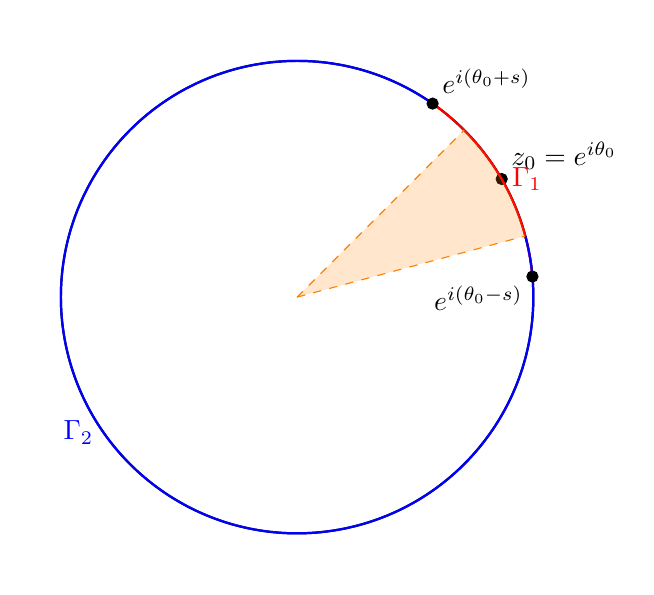
\begin{tikzpicture}
            % Circulo unitario
            \draw[thick] (0,0) circle(3cm);

            % Punto z0
            \filldraw[black] ({3*cos(30)}, {3*sin(30)}) circle (2pt) node[anchor=south west] {$z_0 = e^{i\theta_0}$};

            % Arco alrededor de z0
            \draw[thick, red] ({3*cos(30 + 25)}, {3*sin(30 + 25)}) arc (30 + 25:30 - 25:3cm) node [midway, right] {$\Gamma_1$};

            % Arco complementario
            \draw[thick, blue] ({3*cos(30 + 25)}, {3*sin(30 + 25)}) arc (30 + 25:350 + 25:3cm) node [midway, left] {$\Gamma_2$};

             % Cono desde el centro hasta Gamma_1
            \draw[dashed, orange] (0,0) -- ({3*cos(30 + 15)}, {3*sin(30 + 15)});
            \draw[dashed, orange] (0,0) -- ({3*cos(30 - 15)}, {3*sin(30 - 15)});

            % Relleno naranja del cono
            \fill[orange, opacity=0.2] (0,0) -- ({3*cos(30 + 15)}, {3*sin(30 + 15)}) arc (30 + 15:30 - 15:3cm) -- cycle;

            % Puntos e^i(theta_0 - s) y e^i(theta_0 + s)
            \filldraw[black] ({3*cos(30 - 25)}, {3*sin(30 - 25)}) circle (2pt) node[anchor=north east] {$e^{i(\theta_0 - s)}$};
            \filldraw[black] ({3*cos(30 + 25)}, {3*sin(30 + 25)}) circle (2pt) node[anchor=south west] {$e^{i(\theta_0 + s)}$};

        \end{tikzpicture}
    \end{center}
    Como $\varphi$ es continua en $C(0,1)$, para $\varepsilon' = \frac{\varepsilon}{2} > 0$, existe $s > 0$ tal que si $|\varphi(e^{it}) - \varphi(z_0)| < \varepsilon'$ para $ \forall t \in (\theta_0 - s, \theta_0 + s)$.\\
    Como $\varphi$ es continua en el compacto $C(0,1)$, es acotada, luego existe $M > 0$ tal que $|\varphi(e^{it})| \leq M$ para todo $t \in [0,2\pi]$.\\
    Tomemos $\Gamma_1$ al arco de $C(0,1)$ que va desde $e^{i(\theta_0 - s)}$ hasta $e^{i(\theta_0 + s)}$ y $\Gamma_2$ al arco complementario.\\
    Sea $I_1 = \{ t \in [0,2\pi] : e^{it} \in \Gamma_1 \}$ e $I_2 = \{ t \in [0,2\pi] : e^{it} \in \Gamma_2 \}$. Entonces, tenemos que $I_1$, $I_2$ son subintervalos de $[0,2\pi]$ o la union de 2 subintervalos de $[0,2\pi]$.\\
    Sea ahora $K$ el sector circular de $\overline{D}(0,1)$ del dibujo (en naranja).\\
    Como $K$ y $I_2$ son compactos disjuntos, $d(K,I_2) = \min \{ d(e^{it}, K) : e^{it} \in I_2 \} = \rho > 0$.\\
    Por lo que:
    \[
        |e^{it} - z| \geq \rho \quad \forall z \in K, \forall t \in I_2.
    \]
    Tomamos ahora $\delta > 0$ que cumpla $D(z_0,\delta) \cap \overline{D}(0,1) \subset K$, tal que ademas $\delta < ?$.\\
    Entonces si $z= re^{i\theta} \in D(0,1)$ y $|z - z_0| < \delta$, tenemos que $z \in K$ y por lo tanto:
    \[
        |u(z) - \varphi(z_0)| =
        \frac{1}{2\pi} \int_0^{2\pi} P_r(\theta - t) |\varphi(e^{it}) - \varphi(z_0)| dt =
        \frac{1}{2\pi} \left( \int_{I_1} + \int_{I_2} \right) P_r(\theta - t) |\varphi(e^{it}) - \varphi(z_0)| dt \leq
    \]
    \[
        \leq \frac{1}{2\pi} \frac{\varepsilon}{2} \int_{I_1} P_r(\theta - t) dt + \frac{2M}{2\pi} \int_{I_2} P_r(\theta - t) dt \leq
        \frac{\varepsilon}{2} \left( \frac{1}{2\pi} \int_0^{2\pi} P_r(\theta - t) dt \right) + \frac{M}{\pi} \int_{I_2} \frac{1 - |z|^2}{|e^{it} - z|^2} dt \leq
    \]
    \[
        \leq \frac{\varepsilon}{2} + \frac{M}{\pi} \frac{1}{\rho^2} \int_{I_2} (1 - |z|^2) dt <
        \frac{\varepsilon}{2} + \frac{M}{\pi \rho^2} (1 - |z|^2) 2\pi =
        < \frac{\varepsilon}{2} + \frac{2M}{\rho^2} (1 - |z|^2) \leq^*
    \]
    Ahora usemos que:
    \[
    1 - |z|^2 =
    1 - r^2 =
    (1 - r)(1 + r) \leq
    2(1 - r) =
    2(|z_0| - |z|) \leq
    2|z_0 - z| < 2\delta
    \]
    Continuemos ahora con la demostración:
    \[
        \leq^* \frac{\varepsilon}{2} + \frac{4M}{\rho^2} \delta \underbrace{<}_{\frac{4M}{\rho^2} \delta < \frac{\varepsilon}{2}}
        \frac{\varepsilon}{2} + \frac{\varepsilon}{2} = \varepsilon
    \]
    Por lo tanto, hemos probado que si $|z - z_0| < \delta$, entonces $|u(z) - \varphi(z_0)| < \varepsilon$, y como $\varepsilon > 0$ es arbitrario, deducimos que
    \[
        \lim_{z \to z_0} u(z) = \varphi(z_0).
    \]
\end{proof}

Finalmente, podemos concluir que dada $\varphi: C(0,1) \to \mathbb{R}$ continua, la función $u:D(0,1) \to \mathbb{R}$ dada por:
\[
    u(z) := \begin{cases}
        \frac{1}{2\pi} \int_0^{2\pi} P_r(\theta - t) \varphi(e^{it}) dt & \text{ si } z = re^{i\theta} \in D(0,1) \\
        \varphi(z) & \text{ si } z \in C(0,1)
    \end{cases}
\]
Es solución al problema de Dirichlet en $\overline{D}(0,1)$.\\
Además, es única por el corolario $2$ anterior.

Si ahora tomamos un disco cualquiera $\overline{D}(z_0,R) \subset \mathbb{R}^2$ y una función continua $\varphi: C(z_0,R) \to \mathbb{R}$, podemos reducir el problema de Dirichlet en $\overline{D}(z_0,R)$ al problema de Dirichlet en $\overline{D}(0,1)$, usando la transformación afín que lleva $\overline{D}(z_0,R)$ en $\overline{D}(0,1)$ dada por $h(z) = \frac{z - z_0}{R}$. De esta forma, sabemos que existe una funcion $\widetilde{u} : \overline{D}(0,1) \to \mathbb{R}$ solución al problema de Dirichlet en $\overline{D}(0,1)$ para la función continua $\psi: C(0,1) \to \mathbb{R}$ dada por $\psi(w) = \varphi(h^{-1}(w))$ para todo $w \in C(0,1)$. Entonces, la función $u:\overline{D}(z_0,R) \to \mathbb{R}$ es solución al problema de Dirichlet en $\overline{D}(z_0,R)$ para la función continua $\varphi$ si definimos (usando $z = a + re^{i\theta} \implies h(z) = \frac{{z - z_0}}{R} = \frac{r}{R} e^{i\theta}$):
\[
    u(z) =
    \begin{cases}
        \widetilde{u}\left( h(z) \right) = 
        \frac{1}{2\pi} \int_0^{2\pi} \left( \frac{1 - \left( \frac{r}{R} \right)^2}{1 + \left( \frac{r}{R} \right)^2 - 2 \left( \frac{r}{R} \right) \cos(\theta - t)} \right) \psi \left( h(z_0 + Re^{it}) \right) dt & \text{ si } z \in D(z_0,R) \\
        \varphi(z) & \text{ si } z \in C(z_0,R)
    \end{cases} \implies
\]
\[
    u(z) = u(z_0 + r e^{i\theta}) =
    \begin{cases}
        \widetilde{u} \left( h(z) \right) = 
        \frac{1}{2\pi} \int_0^{2\pi} \left( \frac{R^2 - r^2}{R^2 + r^2 - 2rR \cos(\theta - t)} \right) \varphi(z_0 + Re^{it}) dt & \text{ si } z \in D(z_0,R) \\
        \varphi(z) & \text{ si } z \in C(z_0,R)
    \end{cases}
\]